\cleardoublepage
\chapter{Requirement Analysis}\label{sec:reqs}\minitoc\vspace{.5cm}
\index{Requirements}

\section{Introduction}

Industrial networks have typical configurations, types of traffic, and performance requirements that make them distinct and different from
the traditional communication systems, usually adopted by general-purpose applications.
Configurations and topologies of time-sensitive networks for example are functional to the applications they have to serve.\cite{8715451}
So, to make the evaluation of the network more general it needs to take all different structures and topologies into account without favoring a certain case over the other.

The monitoring system is expected to receive heavy loads of real-time data and should guarantee stable functionality under stress-testing.\\
To help acheiving efficient storage of timeseries a relational database supporting full SQL, such as TimescaleDB is chosen.\\

\begin{figure}[H]
    \centering
    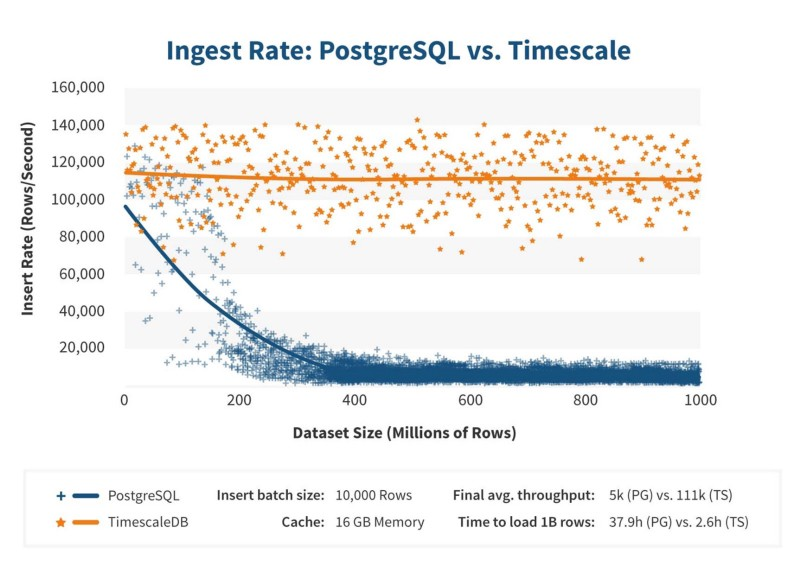
\includegraphics[width=0.9\textwidth]{resources/images/timescaledb_postgres.png}
    \caption{TimescaleDB vs postgres comparison \cite{timescal85}}
    \label{fig:timescaledb-postgres}
\end{figure}

At scale, TimescaleDB exhibits 20x higher insert rates than PostgreSQL, which are relatively constant even as the dataset grows.
PostgreSQL and Timescale start off with relatively even insert performance, but then Postgres's insert rate 
starts to rapidly decline as data volumes approach 100 million rows and only gets worse the higher
the number of row inserts goes.\\

\section{Objectives and Contributions}

This work serves as an experimental and analytical study of monitoring real-time network traffic.\\
This work presents eBPF and XDP as solution to acheive real-time network monitoring assuming little to no background about the subject by the reader.
This dissertation also exposes safety issues related to high-speed communication within a given network.\\
